\section{Aktueller Stand}
\label{sec:chapterexample}

Eine Türsprechanlage, welche Audio und Video überträgt ist keine neue Erfindung. Auf dem Markt existieren bereits verschiedene Lösungen und das schon seit mehreren Jahren. Diese sind aber meistens Analoge Systeme und verfügen über die Vorteile der Digitalisierung nicht. Die Steuerung über eine Mobileapplikation ist bei solche Lösungen aus diesem Grund ausgeschlossen.

\begin{figure}[htb!]
	\begin{center}
		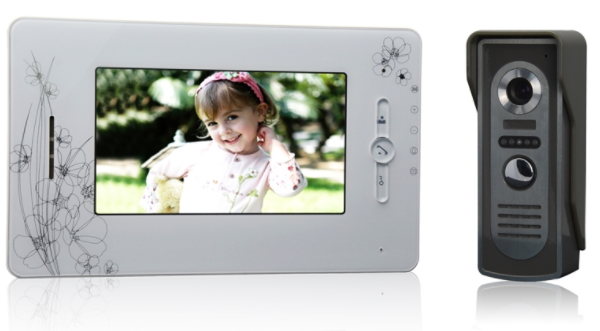
\includegraphics[width=0.66\textwidth]{analog_intercom}
		\caption[Analoge Türsprechanlage mit In-House Display]{Analoge Türsprechanlage mit In-House Display}
		\label{fig:analoge_intercom}
	\end{center}
\end{figure}

In den letzten Jahren sind die ersten Digitale Lösungen mit IP Videoübertragung auf dem Markt gekommen. Die Digitalisierung in diesem Bereich hat es die gigantische Schritten im Bereich der Miniaturisierung und die immer schnellere Internet Zugänge (xDSL, LTE, usw) zu verdanken.

\subsection{Die Herausforderungen der Digitalisierung}
Die Digitalisierung bringt nicht nur Vorteile mit sich. Besonders bei der Video und Audioübertragung. Während eine Analoge Videoübertragung ziemlich mühelos erfolgt muss im Fall eine Digitale Lösung das Video zuerst kodiert und dann dekodiert werden.
\\
Die heutige Kodierung-Algorithmen ermöglichen eine ziemlich schnelle Dekodierung. Mittlerweile hat jeder Smartphone genug Leistung um ein Full-HD Videostream vom Youtube oder Netflix in real-time zu dekodieren. Auf die andere Seite ist die Kodierung ein sehr rechenintensiven Prozess und benötigt sehr viel Leistung.
\\
Jeder der schon mal mit Video-Editing zu tun hatte, weisst, wie viel Zeit die Exportierung eines Video dauern kann.
\\
Die grösste Herausforderung für die real-time Digitale Video/Audio Kommunikation besteht also darin, die Kodierung und Dekodierung der Audio und Video Signal im vernünftigen Zeit durchzuführen. 

\subsection{Marktsituation}
\label{sec:chapterexample}
Der Hauptziel dieses Bachelorarbeit ist, eine Kostengünstige Lösung für eine digitale, flexible und skalierbare Gegensprechanlage. Tatsächlich ist es so, dass die bestehende Lösungen sehr teuer sind. Viele Produkte basieren auf Drittanbieter, SIP Gateways oder andere Elemente die Zusatzkosten verursachen. Das möchten wir alles vermeiden.

\begin{figure}[htb!]
	\begin{center}
		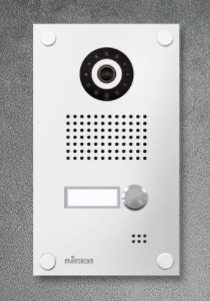
\includegraphics[width=0.33\textwidth]{myintercom}
		\caption[Telecom Behnkle MyIntercom]{Telecom Behnkle MyIntercom}
		\label{fig:myintercom}
	\end{center}
\end{figure}

Eine der günstigsten Produkte den wir finden konnten ist das \textit{"MyIntercom"} von Telecom Behnkle (\seeref{fig:myintercom}). Diese Türklingelanlage ist ziemlich flexibel und bietet die Möglichkeit, mehrere Türen anzuschliessen. Der Preis liegt hier bei zirka 1'600.- CHF pro Türe bei dem Basic-Modell.
\\
\\
 Dank der Aufschwung von Open-Source Hardware wie das Raspberry PI und Real Time Communication Protokolle wie WebRTC muss es möglich sein, kostengünstigere Lösungen zu erarbeiten. Bei den folgenden Kapiteln geht es nun um die effektive Realisierung einem Prototyp, welches die oben genannte Problemen adressiert. 

\newpage